\documentclass[10pt]{amsart}
% \renewcommand{\baselinestretch}{1.27}
\def\today{\number\day\space\ifcase\month\or   January\or February\or
   March\or April\or May\or June\or   July\or August\or September\or
   October\or November\or December\fi\   \number\year}

\usepackage{graphicx}
% \usepackage{epsf}

\theoremstyle{definition}
\newtheorem{thm}{Theorem}[section]
\newtheorem{lem}[thm]{Lemma}
\newtheorem{prp}[thm]{Proposition}
\newtheorem{dfn}[thm]{Definition}
\newtheorem{cor}[thm]{Corollary}
\newtheorem{cnj}[thm]{Conjecture}
\newtheorem{cnv}[thm]{Convention}
\newtheorem{rmk}[thm]{Remark}
\newtheorem{ntn}[thm]{Notation}
\newtheorem{exa}[thm]{Example}
\newtheorem{pbm}[thm]{Problem}
\newtheorem{wrn}[thm]{Warning}
\newtheorem{qst}[thm]{Question}
% \newenvironment{pff}{{\emph{Proof:}}}{\QED}

\newcommand{\beq}{\begin{equation}}
\newcommand{\eeq}{\end{equation}}
\newcommand{\beqr}{\begin{eqnarray*}}
\newcommand{\eeqr}{\end{eqnarray*}}
\newcommand{\bal}{\begin{align*}}
\newcommand{\eal}{\end{align*}}
\newcommand{\bei}{\begin{itemize}}
\newcommand{\eei}{\end{itemize}}
\newcommand{\limi}[1]{\lim_{{#1} \to \infty}}

\newcommand{\af}{\alpha}
\newcommand{\bt}{\beta}
\newcommand{\gm}{\gamma}
\newcommand{\dt}{\delta}
\newcommand{\ep}{\varepsilon}
\newcommand{\zt}{\zeta}
\newcommand{\et}{\eta}
\newcommand{\ch}{\chi}
\newcommand{\io}{\iota}
\newcommand{\te}{\theta}
\newcommand{\ld}{\lambda}
\newcommand{\sm}{\sigma}
\newcommand{\kp}{\kappa}
\newcommand{\ph}{\varphi}
\newcommand{\ps}{\psi}
\newcommand{\rh}{\rho}
\newcommand{\om}{\omega}
\newcommand{\ta}{\tau}

\newcommand{\Gm}{\Gamma}
\newcommand{\Dt}{\Delta}
\newcommand{\Et}{\Eta}
\newcommand{\Th}{\Theta}
\newcommand{\Ld}{\Lambda}
\newcommand{\Sm}{\Sigma}
\newcommand{\Ph}{\Phi}
\newcommand{\Ps}{\Psi}
\newcommand{\Om}{\Omega}

\newcommand{\Q}{{\mathbb{Q}}}
\newcommand{\Z}{{\mathbb{Z}}}
\newcommand{\R}{{\mathbb{R}}}
\newcommand{\C}{{\mathbb{C}}}
% \newcommand{\N}{{\mathbb{N}}}
\newcommand{\N}{{\mathbb{Z}}_{> 0}}
\newcommand{\Nz}{{\mathbb{Z}}_{\geq 0}}
\newcommand{\I}{\infty}

\pagenumbering{arabic}

\newcommand{\inv}{{\mathrm{inv}}}
\newcommand{\tsr}{{\mathrm{tsr}}}
\newcommand{\RR}{{\mathrm{RR}}}
\newcommand{\Tr}{{\mathrm{Tr}}}
\newcommand{\id}{{\mathrm{id}}}
\newcommand{\ev}{{\mathrm{ev}}}
\newcommand{\sint}{{\mathrm{int}}}
\newcommand{\diam}{{\mathrm{diam}}}
\newcommand{\dist}{{\mathrm{dist}}}
\newcommand{\sa}{{\mathrm{sa}}}
\newcommand{\spec}{{\mathrm{sp}}}
\newcommand{\Prim}{{\mathrm{Prim}}}
\newcommand{\diag}{{\mathrm{diag}}}
\newcommand{\supp}{{\mathrm{supp}}}
\newcommand{\rank}{{\mathrm{rank}}}
\newcommand{\sgn}{{\mathrm{sgn}}}
\newcommand{\spn}{{\mathrm{span}}}
\newcommand{\card}{{\mathrm{card}}}
\newcommand{\Aut}{{\mathrm{Aut}}}
\newcommand{\Ad}{{\mathrm{Ad}}}
\newcommand{\Aff}{{\mathrm{Aff}}}
\newcommand{\dirlim}{\varinjlim}
% \newcommand{\dirlim}{\displaystyle \lim_{\longrightarrow}}
\newcommand{\invlim}{\varprojlim}
\newcommand{\Mi}{M_{\infty}}

\newcommand{\andeqn}{\,\,\,\,\,\, {\mbox{and}} \,\,\,\,\,\,}
\newcommand{\QED}{\rule{0.4em}{2ex}}
\newcommand{\ts}[1]{{\textstyle{#1}}}
\newcommand{\ds}[1]{{\displaystyle{#1}}}
\newcommand{\ssum}[1]{{\ts{ {\ds{\sum}}_{#1} }}}

\newcommand{\ca}{C*-algebra}
\newcommand{\ct}{continuous}
\newcommand{\cfn}{continuous function}
\newcommand{\pj}{projection}
\newcommand{\mf}{manifold}
\newcommand{\diff}{diffeomorphism}
\newcommand{\nbhd}{neighborhood}
\newcommand{\cpt}{compact Hausdorff}
\newcommand{\cms}{compact metric space}
\newcommand{\hm}{homomorphism}
\newcommand{\hme}{homeomorphism}
\newcommand{\mh}{minimal homeomorphism}
\newcommand{\so}{solenoid}
\newcommand{\geso}{general solenoid}
\newcommand{\gpso}{group solenoid}
\newcommand{\wolog}{without loss of generality}
\newcommand{\Wolog}{Without loss of generality}
\newcommand{\Tfae}{The following are equivalent}
\newcommand{\tfae}{the following are equivalent}
\newcommand{\ifo}{if and only if}
\newcommand{\rsha}{recursive subhomogeneous algebra}
\newcommand{\Rsha}{Recursive subhomogeneous algebra}
\newcommand{\rshd}{recursive subhomogeneous decomposition}
\newcommand{\mops}{mutually orthogonal \pj s}
\newcommand{\tdim}{topological dimension}
\newcommand{\mms}{maximum matrix size}
\newcommand{\tgca}{transformation group \ca}
\newcommand{\Ei}{Elliott invariant}

\title[Random unitary matrices]{Notes,
questions, and numerical experiments with
random unitary matrices}

\author{N.~Christopher Phillips}

\address{Department of Mathematics, University  of Oregon,
       Eugene OR 97403-1222, USA.}

% \subjclass{Primary ; Secondary .}
\thanks{Research
      partially supported by NSF grants DMS-9706850
      and DMS-0701076.}
\date{14~November 2012}

\begin{document}

\maketitle

This is a very roughly written collection of information
collected that is related to questions such as the following:
Given two random large unitary matrices,
how close are they likely to be to being unitarily equivalent?
Given two random approximately commuting large unitary matrices,
how likely are they to be close to exactly commuting unitary matrices?

A suggested general reference for random matrices,
which I have not seen, is~\cite{Mh}.
I have been warned that the proofs are not always rigorous.

Throughout, unless otherwise specified,
matrices will have complex entries.
We denote the set of $n \times n$ matrices by~$M_n.$
If
\[
a = \big( a_{j, k} \big)_{j, k = 1}^n \in M_n,
\]
then its adjoint $a^*$ is, as usual, the conjugate transpose,
with $(j, k)$ entry equal to ${\overline{a_{k, j}}}.$
A matrix $a \in M_n$ is selfadjoint if $a^* = a,$
unitary if $a^* a = a a^* = 1,$
and normal if $a^* a = a a^*.$
The group of unitary matrices in $M_n$ is denoted by $U (M_n).$
We recall that normal matrices are unitarily diagonalizable:
if $a \in M_n$ is normal, then there is a unitary $u \in M_n$
such that $u a u^*$ (which is the same thing as $u a u^{-1}$)
is diagonal.
The diagonal entries are, of course, the eigenvalues of~$a.$

We identify $M_n$ with the algebra of linear maps from $\C^n$ to~$\C^n$
in the usual way.
We write an element $\xi \in \C^n$
in coordinates as $\xi = (\xi_1, \xi_2, \ldots, \xi_n)$
with $\xi_1, \xi_2, \ldots, \xi_n \in \C,$
often without explicitly saying that the $\xi_k$ are the coordinates
of~$\xi.$
On~$\C^n,$ we use the usual Euclidean norm:
if $\xi \in \C^n,$
then
\[
\| \xi \|_2 = \sqrt{ | \xi_1 |^2 + | \xi_2 |^2 + \cdots + | \xi_n |^2}.
\]
The scalar product of $\xi, \et \in \C^n$ is
\[
\langle \xi, \et \rangle
  = \xi_1 {\overline{\et_1}}
      + \xi_2 {\overline{\et_2}}
      + \cdots + \xi_n {\overline{\et_n}}.
\]
We have the usual properties; in particular, for $\xi, \et \in \C^n$
we have $\| \xi + \et \|_2 \leq \| \xi \|_2 + \| \et \|_2.$
We sometimes abbreviate $\| \xi \|_2$ to $\| \xi \|.$

We define distances in $M_n$ using the operator norm coming from
the Euclidean norm on~$\C^n.$
That is, for $a \in M_n,$
\[
\| a \|
 = \sup \big\{ \| a \xi \|_2 \colon
      \xi \in \C^n, \, \| \xi \|_2 \leq 1 \big\}.
\]
This expression has the following important properties.
(The first three constitute the definition of a norm on a vector space,
and all four togther constitute the definition of a norm on an algebra.)
\begin{enumerate}
\item\label{Norm-Pos}
If $a \in M_n,$ then $\| a \|$ is a nonnegative real number,
and is zero \ifo\  $a = 0.$
\item\label{Norm-Subadd}
For $a, b \in M_n,$ we have $\| a + b \| \leq \| a \| + \| b \|.$
\item\label{Norm-Homog}
For $a \in M_n$ and $\ld \in \C,$
we have $\| \ld a \| = | \ld | \cdot \| a \|.$
\item\label{Norm-Submult}
For $a, b \in M_n,$ we have $\| a b \| \leq \| a \| \cdot \| b \|.$
\end{enumerate}
It is important to realize that, in general,
we do {\emph{not}} have equality in~(\ref{Norm-Submult}).

We follow the convention, usual in operator algebras,
that the identity matrix (of any size) is denoted by~$1.$
(If it is necessary to specify the size,
we use $1_n$ for the $n \times n$ identity matrix.
Moreover, if $\ld \in \C,$
then $\ld \cdot 1$ is abbreviated to~$\ld.$
Thus, the expression which would typically be written
$\ld I - a$ in a linear algebra course becomes $\ld - a.$

% ???
Warning:
Large parts of this file have not been proofread at all,
and some references are incomplete or missing entirely.
Some additional information has been added in the last section,
and not yet properly incorporated into the main text.

\section{Approximate unitary equivalence}\label{Sec:AUE}

Roughly speaking, the question is as follows.
This question was raised about 10 years ago,
and I don't know for sure that it has not been answered since.

\begin{qst}\label{Q-aue-inf}
Let $u$ and $v$ be randomly chosen (independent and uniform
with respect to Haar measure) unitary matrices of the same large
size~$n.$
How close are they likely to be to being unitarily equivalent?
That is, find a bound $\dt_n$ such that, with high
probability, there is a unitary $z$ such that
$\| z u z^* - v \| < \dt_n.$
\end{qst}

The number
$\inf_{z \in U (M_n)} \| z u z^* - v \|$ has a simple
description in terms of the eigenvalues of $u$ and~$v,$
based on the fact that both are unitarily diagonalizable.
Specifically, let $\ld_1, \ld_2, \dots, \ld_n$ be the
eigenvalues of $u,$ repeated according to multiplicity,
and let $\mu_1, \mu_2, \dots, \mu_n$ be the
eigenvalues of~$v,$ repeated according to multiplicity.
Then there are unitaries $x$ and $y$ such that
\[
x u x^* = \diag (\ld_1, \ld_2, \dots, \ld_n)
\andeqn
y v y^* = \diag (\mu_1, \mu_2, \dots, \mu_n)
\]
(diagonal matrices with the specified entries on the diagonal).
One easily checks that
\[
\| (y^* x) u (y^* x)^* - v \|
 = \| \diag (\ld_1, \ld_2, \dots, \ld_n) -
            \diag (\mu_1, \mu_2, \dots, \mu_n) \|
 = \max_{1 \leq k \leq n} | \ld_k - \mu_k |.
\]
So one should choose the listing so as to minimize the maximum
of the errors on the right.
Given a specific listing, this means applying a permutation
to one of the lists.
In fact, this gives the best possible result for $\| z u z^* - v \|$
for arbitrary unitaries~$z.$
In the following theorem,
$S_n$ denotes the symmetric group on $n$~letters,
that is, the set of bijections of $\{ 1, 2, \ldots, n \}.$

Part~(\ref{T-Bhatia-1}) of the following theorem is
Theorem 13.6 of~\cite{Bh}.
Something that approaches Part~(\ref{T-Bhatia-2})
is in a second proof of that theorem,
in Section~17 of~\cite{Bh}.
I believe it can be proved by a combinatorial argument
using only Part~(\ref{T-Bhatia-1}),
but I have not checked.

\begin{thm}\label{T-Bhatia}
Let $n \in \N,$ and let $u, v \in M_n$ be unitaries.
Let
\[
\ld_1, \ld_2, \dots, \ld_n
\andeqn
\mu_1, \mu_2, \dots, \mu_n
\]
be the eigenvalues of $u$ and~$v,$
repeated according to multiplicity.
\begin{enumerate}
\item\label{T-Bhatia-1}
We have
\[
\inf_{z \in U (M_n)} \| z u z^* - v \| =
 \min_{\sm \in S_n}
              \max_{1 \leq k \leq n} | \ld_k - \mu_{\sm (k)} |.
\]
\item\label{T-Bhatia-2}
If the eigenvalues $\ld_1, \ld_2, \dots, \ld_n$ are listed
in cyclic order around the unit circle, then the permutation $\sm$
which gives the minimum in~(\ref{T-Bhatia-1}) has the property that
$\mu_{\sm (1)}, \mu_{\sm (2)}, \dots, \mu_{\sm (n)}$ are listed
in cyclic order around the unit circle.
\end{enumerate}
\end{thm}

The problem with Part~(\ref{T-Bhatia-2})
is that there is no immediate way to determine the starting
point of the cyclic order to use for
$\mu_{\sm (1)}, \mu_{\sm (2)}, \dots, \mu_{\sm (n)}.$

It turns out that the eigenvalues of random unitaries
tend to be much more uniformly distributed around the unit
circle than independent randomly chosen complex numbers of
absolute value~$1.$
(See, for example, Section~IV of~\cite{Dy},
although this is not the original reference for the
random unitary matrices.)
% The reference should be improved. ???
Compare Figures~\ref{Fig:UnifIndepRand100}
and~\ref{Fig:EVOfRandUnitary100}.
This means that the number $\dt_n$ in Question~\ref{Q-aue-inf}
is smaller than it would be if the distribution of eigenvalues were
close to random.

\begin{figure}[htp]
\centering
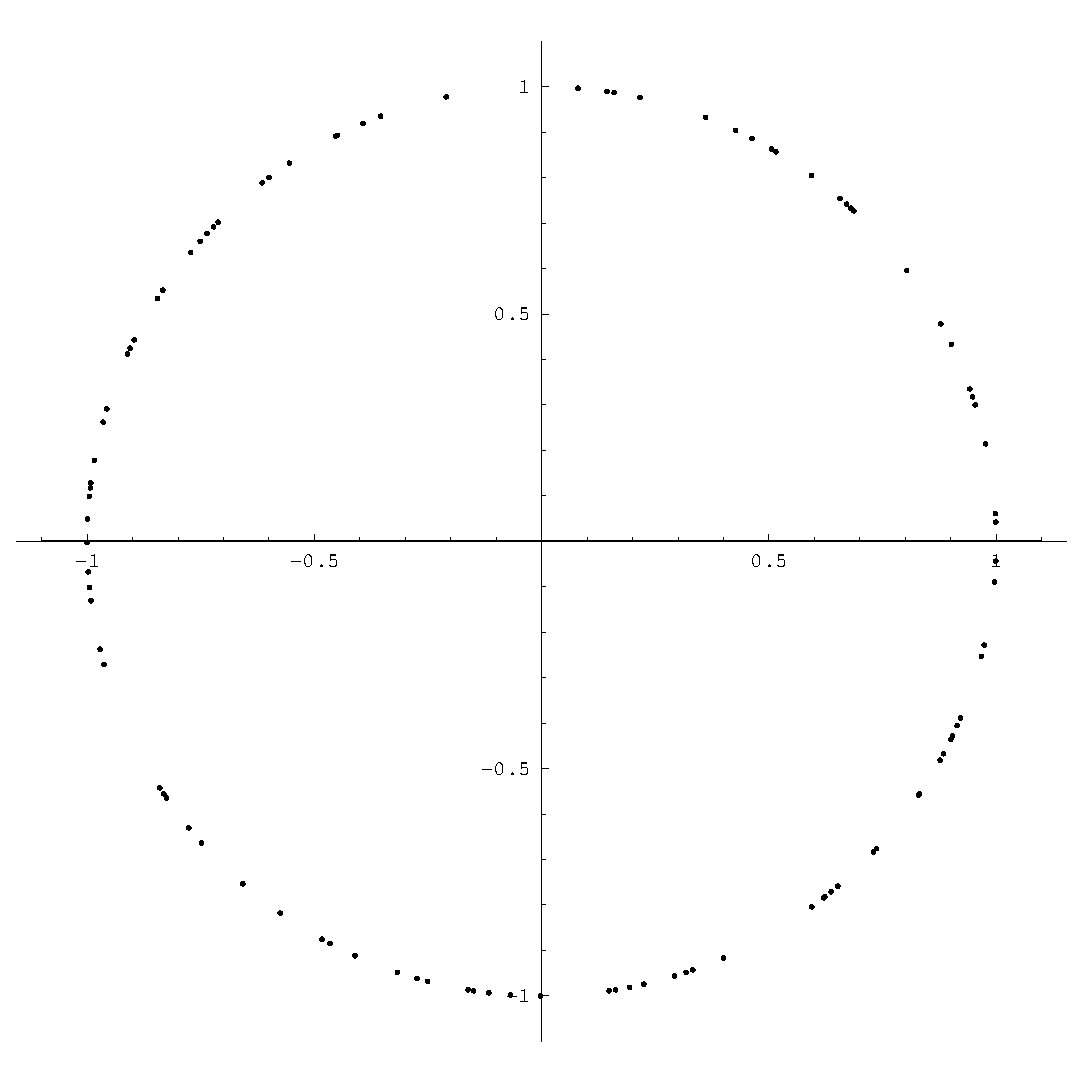
\includegraphics[width=3in]{UnifIndepRand100}
\caption{$100$ independent uniform random points on the unit
   circle.}\label{Fig:UnifIndepRand100}
\end{figure}


\begin{figure}[htp]
\centering
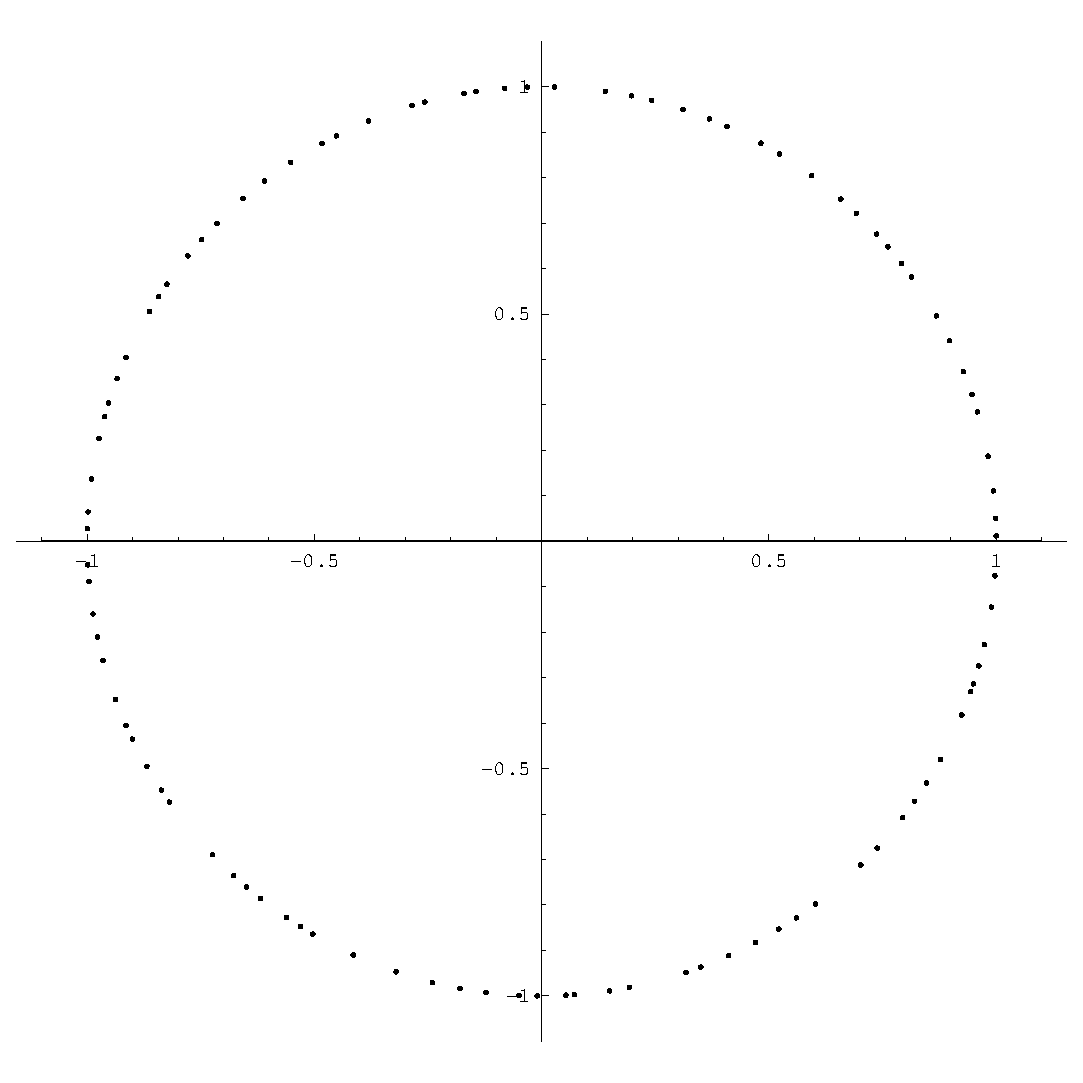
\includegraphics[width=3in]{EVOfRandUnitary100}
\caption{Eigenvalues of a random unitary of size
  $100.$}\label{Fig:EVOfRandUnitary100}
\end{figure}

%	\noindent
%	\center{\textbf{Eigenvalues of a random unitary of size 100}}
%	\vspace{3cm}
%	\nopagebreak
%	% {\epsfxsize=7in \epsffile{EVOfRandUnitary100.eps} }
%	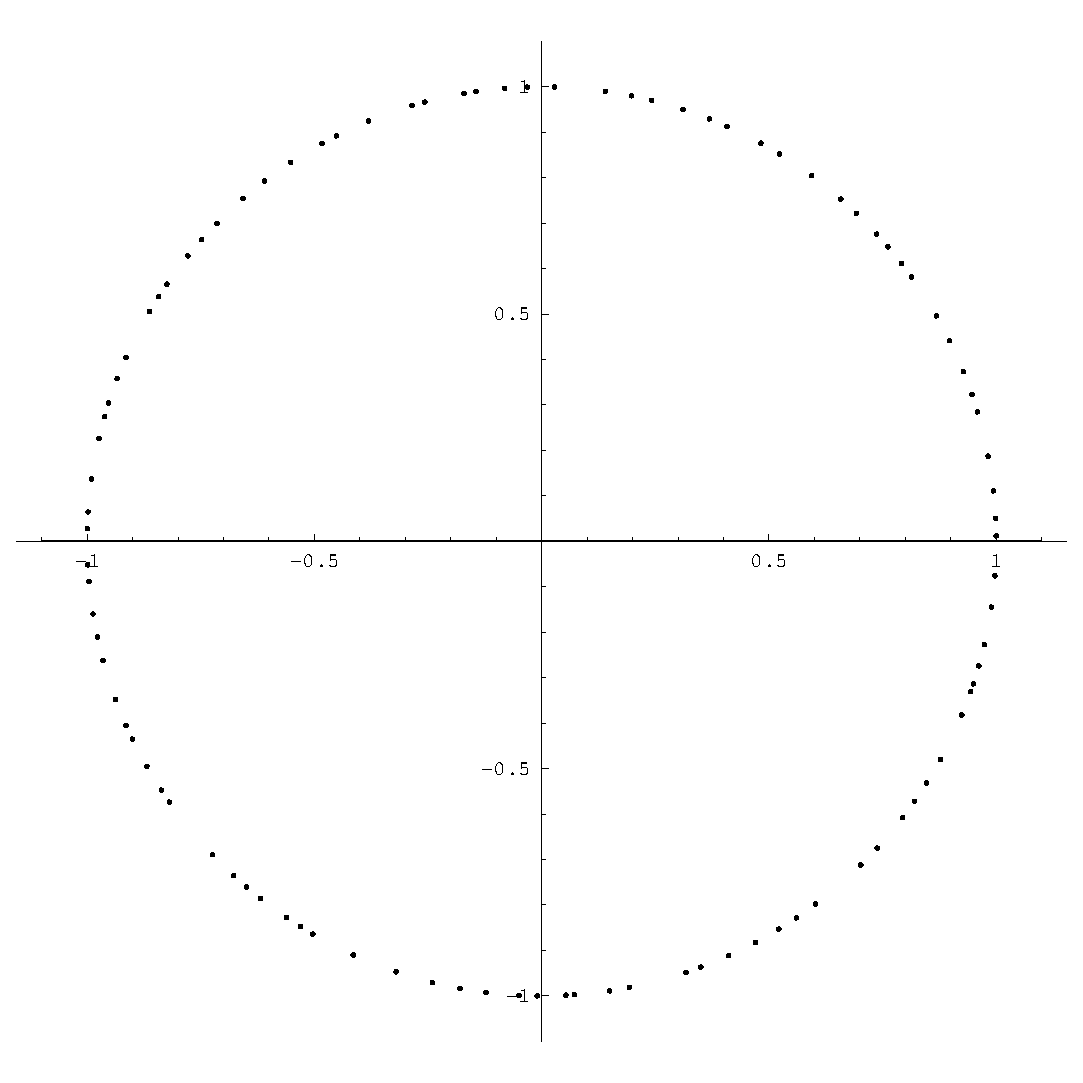
\includegraphics[width=4in]{EVOfRandUnitary100}

%	\noindent
%	\center{\textbf{100 independent uniform random points on the unit circle}}
%	\vspace{3cm}
%	\nopagebreak
%	% {\epsfxsize=7in \epsffile{UnifIndepRand100.eps} }
%	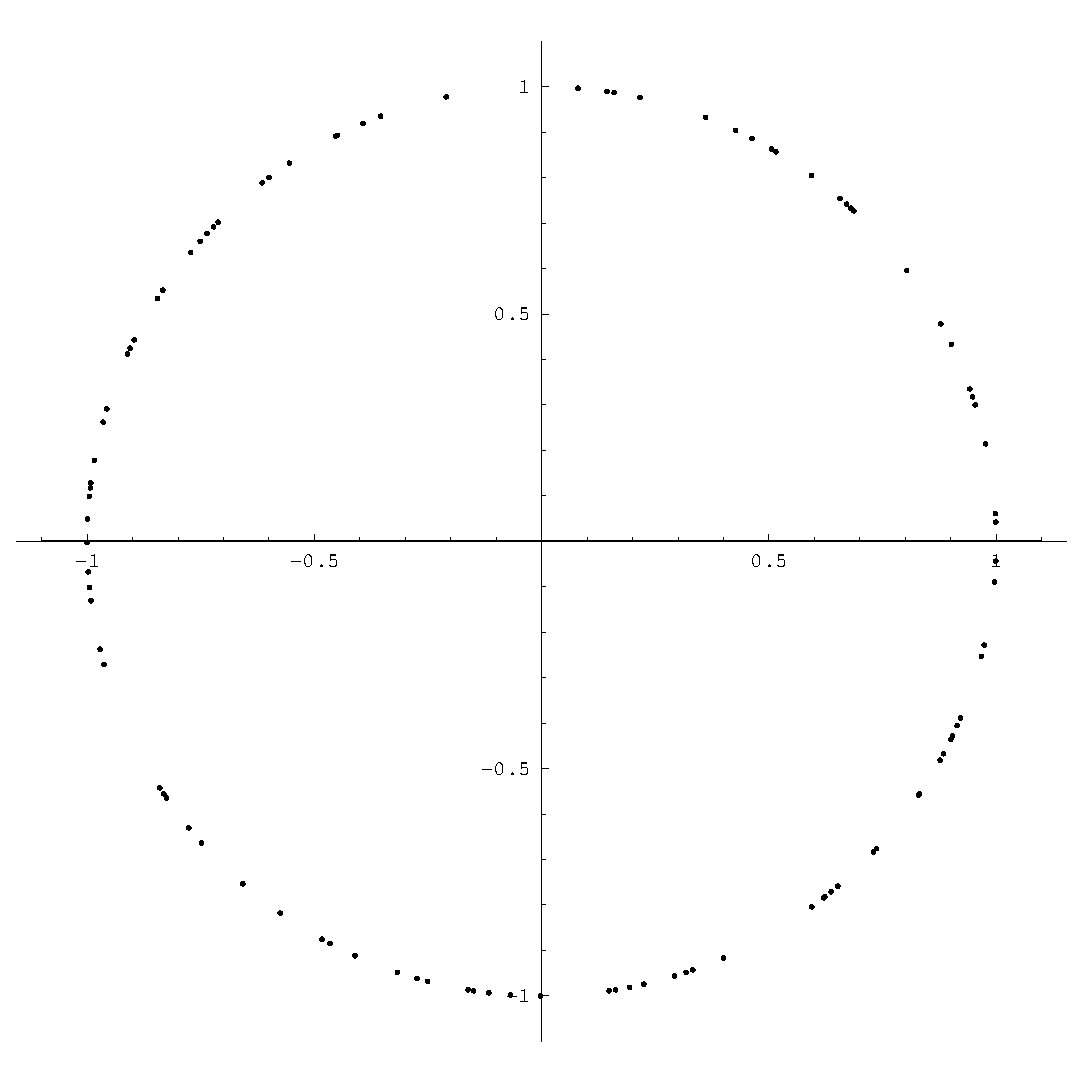
\includegraphics[width=4in]{UnifIndepRand100}

A numerical experiment related to Question~\ref{Q-aue-inf}
(or to other questions described here)
requires a method of constructing
uniformly distributed random unitaries.
Fortunately,
this is fairly easy.
One starts by choosing $2 n^2$ real numbers,
say $\af_{j, k}$ and $\bt_{j, k}$ for $j, k = 1, 2, \ldots, n,$
each independently chosen from the standard normal distribution.
One uses these to construct $n^2$ elements of~$\C^n$:
\begin{align*}
\xi_1 & = \big( \af_{1, 1} + \bt_{1, 1} i, \,
              \af_{2, 1} + \bt_{2, 1} i, \, \ldots, 
              \af_{n, 1} + \bt_{n, 1} i \big),  \\
\xi_2 & = \big( \af_{1, 2} + \bt_{1, 2} i, \,
              \af_{2, 2} + \bt_{2, 2} i, \, \ldots, 
              \af_{n, 2} + \bt_{n, 2} i \big), \\
& \ldots,  \\
\xi_n & = \big( \af_{1, n} + \bt_{1, n} i, \,
              \af_{2, n} + \bt_{2, n} i, \, \ldots, 
              \af_{n, n} + \bt_{n, n} i \big).
\end{align*}
Then one applies the Gram-Schmidt procedure to convert
$\xi_1, \xi_2, \ldots, \xi_n$ to an orthonormal basis:
\begin{align*}
& \et_1 = \left( \frac{1}{\| \xi_1 \|} \right) \xi_1,  \\
& \et_2^{(0)} = \xi_2 - \langle \xi_2, \et_1 \rangle \et_1,  \\
& \et_2
 = \left( \frac{1}{\big\| \et_2^{(0)} \big\|} \right) \et_2^{(0)},  \\
& \et_3^{(0)} = \xi_3
              - \langle \xi_3, \et_1 \rangle \et_1
              - \langle \xi_3, \et_2 \rangle \et_2,  \\
& \et_3
 = \left( \frac{1}{\big\| \et_3^{(0)} \big\|} \right) \et_3^{(0)},  \\
& \ldots,  \\
& \et_n^{(0)} = \xi_n
              - \langle \xi_n, \et_1 \rangle \et_1
              - \langle \xi_n, \et_2 \rangle \et_2
              - \cdots
              - \langle \xi_n, \et_{n - 1} \rangle \et_{n - 1},  \\
& \et_n
 = \left( \frac{1}{\big\| \et_n^{(0)} \big\|} \right) \et_n^{(0)}.  \\
\end{align*}
Now get the random unitary as the $n \times n$ matrix chose columns
are $\et_1, \et_2, \ldots, \et_n.$
(It is just as good to take these to be the rows instead
of the columns.)

In principle, it is possible that the elements
$\xi_1, \xi_2, \ldots, \xi_n$ are linearly dependent,
so that the Gram-Schmidt process can't be carried out.
In theory, this happens with probability zero,
so can be ignored.

It might be interesting to compare the asymptotics of approximate
unitary equivalence of random unitaries with the asymptotics
of the result of applying the matching of Theorem~\ref{T-Bhatia}
to collections of randomly chosen points on the circle.
(Again,
this might turn out to be known.)

\section{The asymptotics of the smallest gap}\label{Sec:SmallestGap}

The problem discussed here was motivated by an approach to
the problem discussed in Section~\ref{Sec:ApproxComm}
(the theoretical version of the idea in Remark~\ref{R-OneDiag}),
but it isn't at all clear that it is actually helpful.

\begin{qst}\label{Q-LargestGap}
How does the expected value of the smallest gap between eigenvalues
of a random $n \times n$ unitary matrix
behave as $n \to \infty$?
\end{qst}

To discuss this, it is convenient to have some notation.

\begin{dfn}\label{D-EVGap}
Let $n \in \N,$ and let $u \in M_n$ be unitary.
Define the {\emph{smallest eigenvalue gap}} $\gm (u)$ of~$u$
to be
\begin{align*}
& \gm (u) = \min \big( \big\{ | \ld_1 - \ld_2 | \colon
         {\mbox{there are linearly independent $\xi_1, \xi_2 \in \C^n$}}
             \\
& \hspace*{37ex}      {\mbox{such that $u \xi_1 = \ld_1 \xi_1$
               and $u \xi_2 = \ld_2 \xi_2$}} \big\}.
\end{align*}
\end{dfn}

If all the eigenvalues of $u$ have multiplicity one,
then $\gm (u)$ is the smallest difference of distinct eigenvalues.
If $u$ has an eigenvalue of multiplicity more than one,
then $\gm (u) = 0.$
In particular,
the minimum in the definition of $\gm (u)$
is over a finite set.

\begin{dfn}\label{D-ExptGap}
For $n \in \N,$
define the {\emph{expected smallest eigenvalue gap}}
$\gm_n$ to be the expected value of $\gm (u_n)$ as
$u$ varies over the $n \times n$ unitary matrices,
with the uniform distribution.
\end{dfn}

We want to know about the behavior of $\gm_n$ as $n \to \I,$
and related questions.
The obvious thing to observe is that an $n \times n$ unitary $u$
has $n$ eigenvalues,
and the largest possible value of $\gm (u)$ is obtained if they are
equally spaced around the circle.
Therefore $\gm_n < 2 \pi / n.$
How much less than $2 \pi / n$ is it?

A good answer would be to find a number $r > 0$ for which there
is a constant $C > 0$ such that
$\gm_n$ behaves like $C n^{- r}$ as $n \to \I.$
That is,
\[
C = \limi{n} \frac{\gm_n}{n^{- r}}
\]
exists.
This may well be too much to hope for; perhaps the best one can do
is find $r > 0$ such that for every $\ep > 0$ we have
\[
\limi{n} \frac{\gm_n}{n^{- r - \ep}} = \I
\andeqn
\limi{n} \frac{\gm_n}{n^{- r + \ep}} = 0.
\]
One might also ask for something slightly different:
to find $r > 0$
for which there
is a constant $C > 0$ such that,
as $n$ gets large, for a random $n \times n$ unitary matrix~$u$
the probability that $\gm (u) < C n^{-r}$
goes to zero.

According to my understanding of discussions with Chris Sinclair,
problems of this nature fall in the area known as ``order statistics'',
and in principle there are methods for obtaining an answer
from the (known) joint distribution of the eigenvalues.
It is possible that the answer is even published,
although I have not seen anything like this.
% ??? More is needed here.

What I am suggesting here is to try to learn something about
the behavior of $\gm_n$ through numerical experiments.
One could, for example,
for small $n$ estimate numerically the number $\gm_n$
by choosing many random $n \times n$ unitary matrices~$u$
and finding $\gm (u)$ for each of them.
Or one could similarly estimate the number $\rh_n$
such that the probability that a
random $n \times n$ unitary matrix $u$ has $\gm (u) < \rh_n$
is $\frac{1}{2}.$
Probably $\gm_n$ and $\rh_n$ behave very similarly,
but this is not guaranteed.

It would be interesting to compare $\gm_n$ (and $\rh_n$)
with the analogous quantities obtained
using sets of $n$ independent randomly chosen points
on the circle instead of the eigenvalues of randomly
chosen $n \times n$ unitary matrices.
(Presumably methods of order statistics could give some
theoretical results here.)
% ??? More is needed here.

\section{Approximately commuting unitary matrices}\label{Sec:ApproxComm}

The following theorem is due to Huaxin Lin~\cite{Ln}.
A much easier proof was provided by Friis and R{\o}rdam~\cite{FR},
and some explicit estimates
and methods for actually finding
the nearby commuting matrices can be found in~\cite{Hs}.

\begin{thm}\label{SA}
% {\tt (Label SA)}
For every $\ep > 0$ there is $\dt > 0$ such that the following holds.
% Let $n$ be a positive integer, and let $a_1, \, a_2 \in (M_n)_{\sa}$
Let $n$ be a positive integer, and let $a_1, \, a_2 \in M_n$
be selfadjoint and
satisfy
\[
\| a_1 \| \leq 1, \,\,\,\,\,\, \| a_2 \| \leq 1, \andeqn
\| a_1 a_2 - a_2 a_1 \| < \dt.
\]
% Then there exist $b_1, \, b_2 \in (M_n)_{\sa}$
Then there exist selfadjoint $b_1, \, b_2 \in M_n$
such that
\[
\| b_1 \| \leq 1, \,\,\,\,\,\, \| b_2 \| \leq 1, \,\,\,\,\,\,
\| a_1 - b_1 \| < \ep,  \,\,\,\,\,\, \| a_2 - b_2 \| < \ep,
\andeqn b_1 b_2 = b_2 b_1.
\]
\end{thm}

The restriction $\| a_1 \|, \, \| a_2 \| \leq 1$ is necessary because
the norm of the commutator scales differently than the norms of the
elements.
The most important point here is that $\dt$ depends only on~$\ep,$
not on~$n.$
This theorem solved a long standing open problem.

If one replaces selfadjoint matrices with unitaries, the analogous
result is false.
The standard counterexample is provided by the well known
Voiculescu matrices, and was first found in~\cite{Vc}.
Let $n > 0,$ and let $\zt_n = \exp (2 \pi i / n),$ a primitive
$n$-th root of~$1.$
Then the Voiculescu matrices are given by
% \[
% w_n = \left( \begin{array}{ccccccc}
%      1 & 0 & 0 & \cdots & \cdots & 0 & 0 \\
%      0 & \zt_n & 0 & \cdots & \cdots & 0 & 0 \\
%      0 & 0 & \zt_n^2 & \cdots & \cdots & 0 & 0 \\
%      \vdots & \vdots & \vdots & \ddots &        & \vdots & \vdots \\
%      \vdots & \vdots & \vdots &        & \ddots & \vdots & \vdots \\
%      0 & 0 & 0 & \cdots & \cdots & \zt_n^{n - 2} & 0 \\
%      0 & 0 & 0 & \cdots & \cdots & 0 & \zt_n^{n - 1} \\
%    \end{array} \right)
% \andeqn
% s_n = \left( \begin{array}{ccccccc}
%      0 & 0 & 0 & \cdots & \cdots & 0 & 1 \\
%      1 & 0 & 0 & \cdots & \cdots & 0 & 0 \\
%      0 & 1 & 0 & \cdots & \cdots & 0 & 0 \\
%      \vdots & \vdots & \vdots & \ddots &        & \vdots & \vdots \\
%      \vdots & \vdots & \vdots &            & \ddots & \vdots & \vdots \\
%      0 & 0 & 0 & \cdots & \cdots & 0 & 0 \\
%      0 & 0 & 0 & \cdots & \cdots & 1 & 0 \\
%    \end{array} \right).
% \]
\[
w_n = \left( \begin{array}{cccccc}
     1 & 0 & 0 & \cdots & \cdots &  0 \\
     0 & \zt_n & 0 & \cdots & \cdots &  0 \\
     0 & 0 & \zt_n^2 & \cdots & \cdots &  0 \\
     \vdots & \vdots & \vdots & \ddots &        &  \vdots \\
     \vdots & \vdots & \vdots &        & \ddots & \vdots \\
      0 & 0 & 0 & \cdots & \cdots &  \zt_n^{n - 1} \\
   \end{array} \right)
\andeqn
s_n = \left( \begin{array}{cccccc}
     0 & 0 &  \cdots & \cdots & 0 & 1 \\
     1 & 0 &  \cdots & \cdots & 0 & 0 \\
     0 & 1 &  \cdots & \cdots & 0 & 0 \\
     \vdots &  \vdots & \ddots &        & \vdots & \vdots \\
     \vdots &  \vdots &            & \ddots & \vdots & \vdots \\
     0 & 0 &  \cdots & \cdots & 1 & 0 \\
   \end{array} \right).
\]
That is, $w_n$ is a diagonal matrix with the powers of $\zt_n$ down the
diagonal, and $s_n$ is a cyclic shift.
It is easy to check that
\[
\| s_n v_n - v_n s_n \| = \| s_n v_n s_n^* - v_n \| = | \zt_n - 1 |
    < 2 \pi / n.
\]
It can be shown that there do not exist unitaries $x$
close to $v$ and $y$ close to $s$ such that $x y = y x.$
Some of the theory behind this is discussed below, but we point out here
an elementary proof (using nothing beyond winding numbers)
in~\cite{EL1} which shows that if $x, \, y \in M_n$ are any matrices
(not necessarily unitary, or even normal) with  $x y = y x,$ and
if $n \geq 7,$ then
\[
\max \big( \| x - v_n \|, \, \| y - s_n \| \big)
       \geq \sqrt{2 - | \zt_n - 1 |} - 1.
\]

% Although other questions will be mentioned as they come up, the
The
main point of this section is to discuss the following question
and possible numerical experiments to test it.
The question will be formulated more precisely below.

\begin{qst}\label{ACProb1}
Is it true that ``most'' pairs of approximately commuting large
unitary matrices
are close to pairs of commuting unitary matrices?
\end{qst}

The answer to this question is not known.

Given two approximately commuting unitaries, one can test
whether they are close to commuting unitaries with the help
of some invariants.
See~\cite{EL2} for a discussion of several of these,
and~\cite{Ex} for one improvement.
The most easily computable one (both theoretically
and numerically) is the winding number invariant, defined
as follows.

\begin{dfn}\label{D-WndNo}
Let $n > 0,$ and let $u, \, v \in U (M_n)$ satisfy
$\| u v - v u \| < 2.$
We define the {\emph{winding number invariant}} $\om (u, v)$ to be the
winding number about $0$ of the closed path in $\C \setminus \{ 0 \}$
given by $\af \mapsto \det \big( (1 - \af) u v + \af v u \big)$ for
$\af \in [0, 1].$
\end{dfn}

The condition $\| u v - v u \| < 2$ ensures that
$\big\| u v - [(1 - \af) u v + \af v u] \big\| < 1$ for
$\af \in \big[ 0, \frac{1}{2} \big]$ and
$\big\| v u - [(1 - \af) u v + \af v u] \big\| < 1$ for
$\af \in \big[ \frac{1}{2}, 1 \big].$
This ensures that $(1 - \af) u v + \af v u$ is always invertible,
so that its determinant really is never zero.

There are also various forms of a K-theoretic invariant
that we call $\kp (u, v).$
Several equivalent versions are given in~\cite{EL2} for
$\| u v - v u \|$ small, and an extension (less elementary)
valid for all $u$ and $v$ with $\| u v - v u \| < 2$ is given
in~\cite{Ex}.
It is shown in~\cite{EL2} and in Theorem~3.2 of~\cite{Ex}
that these invariants
agree with the winding number invariant above.

The winding number invariant is the only obstruction in an
asymptotic sense.

\begin{thm}[Corollary~6.15 of~\cite{ELP}]\label{UThm}
For every $\ep > 0$ there is $\dt > 0$ such that the following holds.
Let $n$ be a positive integer, and let $u_1, \, u_2 \in U(M_n)$
satisfy
\[
\| u_1 u_2 - u_2 u_1 \| < \dt \andeqn \om (u_1, u_2) = 0.
\]
Then there exist $v_1, \, v_2 \in U (M_n)$ such that
\[
\| u_1 - v_1 \| < \ep,  \,\,\,\,\,\, \| u_2 - v_2 \| < \ep,
\andeqn v_1 v_2 = v_2 v_1.
\]
\end{thm}

Unfortunately, we do not know anything about how $\dt$ depends
on $\ep.$
The following is a presumably difficult theoretical problem.

\begin{pbm}\label{PA}
In Theorem~\ref{UThm}, find an explicit formula for a possible
value of $\dt$ in terms of $\ep.$
\end{pbm}

Nevertheless, it seems reasonable to hope that the
winding number invariant gives the right answer when
the norm of the commutator is not too large and the matrix
size is large.
We therefore propose the following numerical experiments:

\begin{pbm}\label{ACProb2}
Determine experimentally whether
``most'' pairs of approximately commuting large
unitary matrices
have winding number invariant equal to zero.
More generally, experimentally estimate the statistical
distribution of the values of the winding number invariant
for pairs of large unitary matrices $(u, v)$ such that
$\| u v - v u \| < 2.$
\end{pbm}

\begin{pbm}\label{ACProb3}
Experimentally estimate the asymptotics of the quantities
in Problem~\ref{ACProb2} as the matrix size becomes large.
For example, for a carefully chosen scaling factor~$\ep_n$
(possibly $\ep_n = \ep / \sqrt{n},$ but this is not clear),
find the asymptotic distribution of the winding number invariant
for pairs of $n \times n$ unitary matrices $(u, v)$ such that
$\| u v - v u \| < \ep_n.$
\end{pbm}

\begin{rmk}\label{R-NumW}
The winding number invariant $\om (u, v)$ of Definition~\ref{D-WndNo}
is in principle numerically computable,
although it is not clear how easily it can be done in practice.
For $\af \in [0, 1]$
set $\gm (\af) = \det \big( (1 - \af) u v + \af v u \big).$
The formula is
\[
\om (u, v)
  = \frac{1}{2 \pi i} \int_{\gm} \frac{1}{\zt} \, d \zt
  = \frac{1}{2 \pi i} \int_0^1 \frac{\gm' (\af)}{\gm (\af)} \, d \af.
\]
Determinants are computed by row reduction.
I don't know whether it is better to numerically estimate
the derivative,
or to derive an algebraic form for it in terms of other
determinants.
There are a number of numerical methods for calculating integrals.
One need not compute the integral very accurately,
since it is known ahead of time that the answer must be an integer.
\end{rmk}

It seems very hard to generate randomly pairs of approximately
commuting unitaries.
One can easily generate random unitaries.
To get a random $n \times n$ unitary matrix,
one simply chooses $2 n^2$ real numbers independently
from the standard normal distribution,
uses them as the real and imaginary parts of the entries
of $n$ vectors in~$\C^n,$
and applies the Gram-Schmidt process to turn these vectors
into an orthonormal basis.

However, most pairs will
not approximately commute,
and the proportion that do
will decrease exponentially with the dimension.

Here are several ideas that, by themselves, don't solve this difficulty,
but which might help.
The first two
came from discussion with Benjamin Morris in Jan.\  2005.

\begin{rmk}\label{R-Metropolis}
The ``Metropolis Algorithm'' is essentially a very general method
for generating random elements of connected sets.
The element depends on some parameters
(here, the $2 n^2$ entries of two $n \times n$ unitary matrices).
Start with an element of the set
(here,
$\{ (u, v) \in U (M_n) \colon \| u v - v u \| < \ep \}$).
Change one of the parameters, chosen at random,
by a random small amount, and push the perturbed matrix back into the
unitary group (using functional calculus).
If the result is still in the set,
replace the old element by the new one;
otherwise, keep the old element.
In a connected set, if this procedure is run long enough,
the distribution will be uniform.
In a very long and thin set,
which is quite possibly what we have,
the time required to approach uniformity will be very large.
One with ``bottlenecks'' may be even worse.
Also, the set of pairs of almost commuting unitaries is not connected;
pairs for which the winding number invariant is different must
be in different connected components.
It is not clear whether the set of pairs of almost commuting unitaries
with fixed winding number invariant is connected.
\end{rmk}

\begin{rmk}\label{R-Doubling}
There is a kind of ``doubling'' method for estimating volumes.
We want to estimate the volume of a set~$S_0,$
known to be contained in some space with finite volume.
We choose a larger set $S_1$ whose volume should be very roughly twice
that of~$S_0.$
Use a Monte Carlo method
to estimate ${\mathrm{vol}} (S_0) / {\mathrm{vol}} (S_1)$
as the conditional probability that a point is in $S_0$ given
that it is in~$S_1.$
Then choose a larger set~$S_2,$ etc.
Probably
one will choose $S_{n + 1}$ to be a suitable neighborhood of~$S_n,$
or else choose the $S_n$ to be suitable neighborhoods of~$S_0.$
\end{rmk}

\begin{rmk}\label{R-OneDiag}
The following refinement should at least substantially speed up
the brute force approach.
Choose a unitary $u_0$ at random, and diagonalize it,
in such a way that the diagonal of the resulting unitary $u$
is the eigenvalues of $u_0$ listed in cyclic order around
the unit circle.
We get $u = z u_0 z^*$ for some unitary~$z.$
Now choose $v$ at random.
The probability that $\| u v - v u \| < \ep,$
and the probability that $u$ and $v$ are close to commuting unitaries,
should be the same as if both were chosen completely at random.
The reason is that if $v$ is chosen uniformly at random,
then $z^* v z$ is also random and uniformly distributed.

For a very large proportion of the choices of~$u,$
the diagonal entries will be fairly close to being evenly spaced
around the circle.
Now some easy tests will show that many choices of $v$
do not approximately commute with~$u.$
For example,
if any entry of $v$ a significant distance from the diagonal
is fairly large,
it probably follows that $\| u v - v u \|$ can't be very small.
(Lemma~4.3 of~\cite{St} shows that two almost commuting
unitary matrices are simultaneously approximately diagonalizable,
but this probably doesn't help much,
since it isn't clear how the basis is related to the given one.
The main result of~\cite{Os} gives some information
about what happens when the diagonal entries are not evenly spaced.)

Presumably one can get reasonable numerical estimates
of probabilities by using many choices of~$u,$
and for each fixed choice of~$u,$
using many choices of~$v.$
In a different direction,
it might be possible to numerically generate eigenvalue lists
for random unitaries directly,
much more quickly than diagonalizing randomly chosen unitaries.
\end{rmk}

\section{Additional information}\label{Sec:Add}

\indent
This section contains
some additional information which has
not yet properly incorporated into the main text.

Marius
Dadarlat's talk slides from the June 2011 CRM conference have various
versions or generalizations of Loring and Exel-Loring formulas for the
K-theoretic obstruction to perturbing almost commuting unitaries to
commuting ones.

\vspace{1ex}

The following is from an email message from Chris Sinclair
of 21~June 2011.

{\textbf{My question:}}
Second, do you know of any way of producing a large number
of lists of eigenvalues chosen from this distribution that is
more efficient than generating a large number of random unitaries
and diagonalizing them? This is wanted for numerical experiments.
It is easy to generate a random unitary in $M_n$: Choose $n$ elements
of $\C^n$ whose real and imaginary parts are independent normally
distributed with the same standard deviation and with mean zero,
and apply Gram-Schmidt to orthonormalize them. But then there is
numerical work to find eigenvalues.

{\textbf{Response:}}
The distribution of eigenvalues is known, so there must be some standard
sampling method which would be applicable.  However, I am not an expert
on this sort of statistics, so I really can't tell you.  Another
possible approach is the following:  Consider the set of polynomials
with all roots on the unit circle.  One can parametrize this set in a
natural way so that the coefficient vectors of such polynomials can be
identified with a subset of $\C^M$
(for some appropriate value of $M$).  The
roots of a polynomial chosen uniformly in this set will have the same
distribution as the eigenvalues of a random unitary matrix.  (I hope I
am remembering this correctly.  You might look at
http://arxiv.org/pdf/math/0511397).  One could then do some sort of
selection/rejection regime to select such a polynomial uniformly.  There
are bounds for the coefficients, which makes the search space bounded. 
See:

Sinclair, C. D., \& Vaaler, J. D. (2008).
Self-Inversive Polynomials with
All Zeros on the Unit Circle. In J. McKee \& C. Smyth (Eds.), Number
Theory and Polynomials: Proceedings of the workshop held at {B}ristol
{U}niversity, {B}ristol, {A}pril 3--7, 2006, London Mathematical Society
Lecture Note Series (Vol. 352, pp. xiv+349). Cambridge: Cambridge
University Press. doi:10.1017/CBO9780511721274

I'm not sure this method will be useful however, since the volume of the
set of such polynomials is rather small, especially when the degree is
large.


{\textbf{My question:}}
Third, do you know a citable reference for generating
random unitaries numerically?

{\textbf{Response:}}
No.

{\textbf{My question:}}
Fourth, have you ever heard of any work on the following
question: Given two $n \times n$ random unitaries $u$ and $v,$
what are the
asymptotics of how close they are to being unitarily equivalent?
That is, consider, say, the expected value of the minimum of
$\| u - z v z* \|$ over all unitaries $z,$ and ask how this quantity
behaves as $n \to \infty.$ (It is known that the minimum of
$\| u - z v z* \|$ depends only on the eigenvalues of $u$ and $v.$)

{\textbf{Response:}}
Huaxin asked me a question along these lines once.  However, I haven't
had the time to really consider it.  I know of no results in this
direction, though I'm not really an expert in circular ensembles.

{\textbf{My question:}}
As a possible contrast with some of this, is anything
known about the asymptotics of the following: Choose n points on
the circle, independently and uniformly according to arc length
measure. What happens to the expected value of the minimum distance
between two of these point, as $n \to \infty$?

{\textbf{Response:}}
This must be known, or at least knowable.  This follows under the guise
of order statistics.  Once one knows the distribution of the gaps
between points, then one can "easily" get the distribution of the
smallest gap and therefore the expectation.  This would be a good
exercise in order statistics.  Determining the asymptotics of this
quantity would then, in principle, be doable.  For the Circular Unitary
Ensembles (random unitaries) the asymtptotic distribution of gaps
(scaled so that the expected gap size is, say, 1) is known.  I suspect
the asymptotics of the smallest gap is known too, but I don't know of a
reference off the top of my head.  By universality, the answer must be
the same as for the Gaussian Unitary Ensemble.  You might look in
Mehta's book Random Matrices, which has a wealth of such facts (though
his proofs are often not rigorous).


\begin{thebibliography}{BKR}

\bibitem{Bh} R.~Bhatia,
{\emph{Perturbation Bounds for Matrix Eigenvalues}},
Pitman Research Notes in Math.\  no.~162,
Longman Scientific and Technical, Harlow, Britain, 1987.

\bibitem{ELP}
S.~Eilers, T.~A.\  Loring, and G.~K.\  Pedersen,
{\emph{Morphisms of extensions of C*-algebras: Pushing forward the Busby
        invariant}},
Adv.\  Math.\   {\textbf{147}}(1999), 74--109.

\bibitem{Dy} F.~J.\  Dyson,
{\emph{Statistical theory of the energy levels of complex systems. I}},
J.~Mathematical Phys.\  {\textbf{3}}(1962), 140--156.

% \bibitem[ELP]{ELP}
% S.\   Eilers, T.\  A.\   Loring, and G.\  K.\  Pedersen,
% {\em Stability of anticommutation relations. An application of
%         noncommutative CW complexes},
% J.\  reine angew.\  Math.\   {\bf 499}(1998),  101--143.

\bibitem{Ex} R.~Exel,
{\emph{The soft torus and applications to almost commuting matrices}},
Pacific J.\  Math.\  {\textbf{160}}(1993), 207--217.

\bibitem{EL1} R.~Exel and T.~A.\  Loring,
{\emph{Almost commuting unitary matrices}},
Proc.\  Amer.\  Math.\  Soc.\   {\textbf{106}}(1989),  913--915.

\bibitem{EL2} R.~Exel and T.~A.\  Loring,
{\emph{Invariants of almost commuting unitaries}},
J.~Funct.\  Anal.\  {\textbf{95}}(1991), 364--376.

\bibitem{FR}
P.~Friis and M.~R{\o}rdam,
{\emph{Almost commuting self-adjoint matrices -- a short proof
  of Huaxin Lin's theorem}},
J.~reine angew.\  Math.\   {\textbf{479}}(1996), 121--132.

% \bibitem[GL]{GL} G.\  Gong and H.\  Lin,
% {\em Almost
% multiplicative morphisms and almost multiplicative matrices},
% ???  {\bf }(19??),  .

\bibitem{Hs}  M.~B.\  Hastings,
{\emph{Making almost commuting matrices commute}},
Commun.\  Math.\  Phys.\  {\textbf{291}}(2009), 321--345.

\bibitem{Ln} H.~Lin,
{\emph{Almost commuting selfadjoint matrices and applications}},
pages 193--233 in:
{\emph{Operator Algebras and their Applications
(Waterloo, ON, 1994/1995)}},
Fields Inst.\  Commun.\  vol.~13,
Amer.\  Math.\  Soc., Providence, RI, 1997.

\bibitem{Mh} M.~L.\  Mehta,
{\emph{Random matrices}} (3rd ed.),
Pure and Applied Mathematics (Amsterdam), vol.\  142,
Elsevier/Academic Press, Amsterdam, 2004.

\bibitem{Os} T.~J.\  Osborne,
{\emph{Almost commuting unitaries with spectral gap are near commuting
  unitaries}},
Proc.\  Amer.\  Math.\  Soc.\  {\textbf{137}}(2009), 4043--4048.

\bibitem{St} M.~Steiner,
{\emph{Variations on a theme of Frobenius about almost commuting unitary
  matrices}},
Linear Algebra Appl. {\textbf{400}}(2005), 1--13.

\bibitem{Vc} D.~Voiculescu,
{\emph{Asymptotically commuting finite rank unitary operators
without commuting approximants}},
Acta Sci.\  Math.\  (Szeged) {\textbf{45}}(1983),  429--431.

\end{thebibliography}

\end{document}
